%%%%%%%%%%%%%%%%%%%%%%%%%%
%%% author : Yamada. T %%%
%%% made for TH series %%%
%%%%%%%%%%%%%%%%%%%%%%%%%%

\documentclass[b5paper,10pt,fleqn] {ltjsarticle}

\usepackage[margin=10truemm]{geometry}

\usepackage{pict2e, graphicx}
\usepackage{tikz}
\usetikzlibrary{intersections,calc,arrows.meta}

\usepackage{amsmath, amssymb, amsthm}
\usepackage{ascmac}
\usepackage{comment}
\usepackage{empheq}
\usepackage[shortlabels,inline]{enumitem}
\usepackage{fancybox}
\usepackage{fancyhdr}
\usepackage{here}
\usepackage{lastpage}
\usepackage{listings, jvlisting}
\usepackage{fixdif}

\usepackage{stmaryrd}
\usepackage[listings]{tcolorbox}
%\usepackage{ascolorbox}
\usepackage{titlesec}
\usepackage{ulem}
\usepackage{url}
\usepackage{verbatim}
\usepackage{wrapfig}
\usepackage{xcolor}
\usepackage{luatexja-ruby}
\usepackage{varwidth}
\usepackage[version=3]{mhchem}
\usepackage{wrapfig}


\usepackage{physics2}
	\usephysicsmodule{ab}
	\usephysicsmodule{ab.braket}
	\usephysicsmodule{ab.legacy}
	%\usephysicsmodule{braket}
	\usephysicsmodule{diagmat}
	\usephysicsmodule{xmat}
	\usephysicsmodule{nabla.legacy}
	\usephysicsmodule{qtext.legacy}

\usepackage[ISO]{diffcoeff}
\difdef { f, s } { D }
{ op-symbol = \mathrm{D} }


\newcommand{\mctext}[1]{\mbox{\textcircled{\scriptsize{#1}}}}
\newcommand{\ctext}[1]{\textcircled{\scriptsize{#1}}}
\newcommand{\ds}{\displaystyle}
\newcommand{\comb}[2]{{}_{#1}\mathrm{C}_{#2}}
\newcommand{\hs}{\hspace}
\newcommand{\vs}{\vspace}
\newcommand{\emphvs}{\vspace{1em}\notag\\}
\newcommand{\ora}{\overrightarrow}
\newcommand{\ol}{\overline}
\newcommand{\oramr}[1]{\overrightarrow{\mathrm{#1}}}
\newcommand{\tri}{\triangle}
\newcommand{\mr}{\mathrm}
\newcommand{\mb}{\mathbb}
\newcommand{\mrvec}[1]{\overrightarrow{\mathrm{#1}}}
\newcommand{\itvec}{\overrightarrow}
\newcommand{\bs}{\boldsymbol}
\newcommand{\ra}{\rightarrow}
\newcommand{\Ra}{\Rightarrow}
\newcommand{\lra}{\longrightarrow}
\newcommand{\Lra}{\Longrightarrow}
\newcommand{\la}{\leftarrow}
\newcommand{\La}{\Leftarrow}
\newcommand{\lla}{\longleftarrow}
\newcommand{\Lla}{\Longleftarrow}
\newcommand{\lr}{\leftrightarrow}
\newcommand{\llr}{\longleftrightarrow}
\newcommand{\Llr}{\Longleftrightarrow}
\renewcommand{\deg}{{}^\circ}
\newcommand{\phbox}{\fbox{\phantom{1\hspace{2em}}}}
\newcommand{\boxnum}[1]{\fbox{\phantom{\hspace{1em}}({#1})\phantom{\hspace{1em}}}}
\newcommand{\boxkana}[1]{\fbox{\phantom{\hspace{1em}}{#1}\phantom{\hspace{1em}}}}
\newcommand{\boxkm}[2]{\fbox{\, {#1}\phantom{\hspace{0.2em}} \,  {#2}}}
\newcommand{\hzw}{\hspace{1\zw}}

\renewcommand{\baselinestretch}{1.25}
\parindent=1\zw

%%% TH3-4
\begin{document}
\noindent
\fbox{NewTH1-7} [東京大]

\begin{wrapfigure}{r}{8cm}
    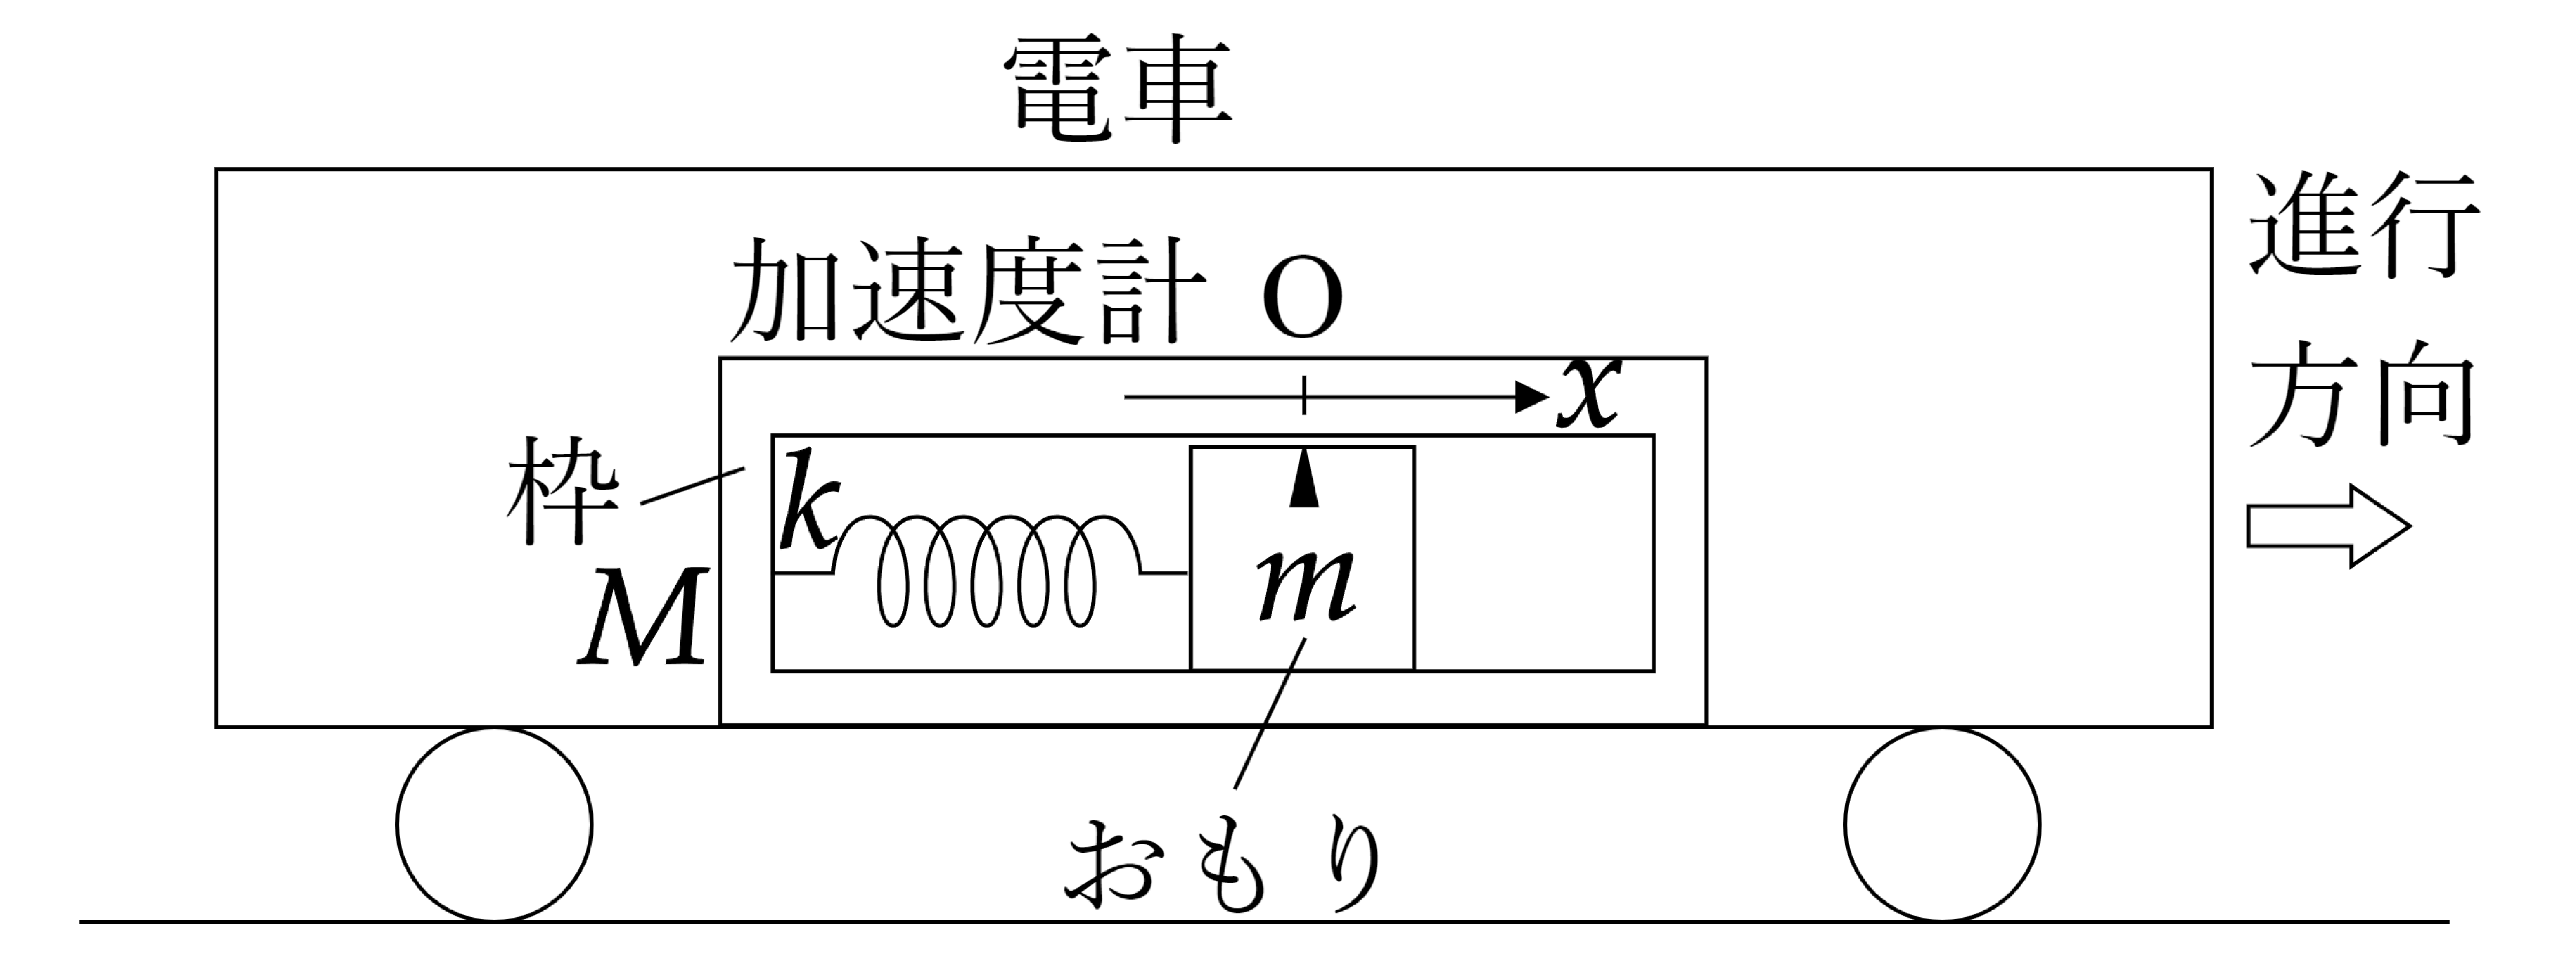
\includegraphics[width=8cm]{fig/fig_1_7_1.pdf}
    \caption{}
\end{wrapfigure}
走行中の電車の中で電車の加速度を測定するために,図1に示すように,質量$m$のおもり,質量$M$の枠,質量の無視できるばね定数$k$のばねからなる加速度計を,電車の床に固定した.
ばねの一端はおもりに固定され,他端は枠の内側に固定されており,おもりは枠の中で直線運動するようになっている.
枠に固定された座標系を考え,この座標系におけるおもりの位置を$x$とする.
ばねが自然の長さの時のおもりの位置を$x = 0$とし,ばねが伸びる向きを$x$軸の正の向きとする.
また,$x$軸の正の向きは,電車の進行方向と一致しているとする.
枠とおもりの間の摩擦は無視でき,おもりが枠の端に接触したり,ばねが縮みきったりすることはないものとして,以下の問いに答えよ.
ただし,重力加速度の大きさを$g$とし,電車の加速度の向きは,電車の進行方向を正として,正負の符号により表すものとする.

\begin{enumerate}[I]
  \item {\hzw}電車が水平でまっすぐなレールの上を走っている場合を考える.
  \begin{enumerate}[label=\textbf{問\arabic*}]
    \item {\hzw}電車が一定の加速度で走っているとき,おもりは枠に対して単振動した.振動の中心の$x$座標を$x_0$とするとき,電車の加速度を$m$,$k$,$x_0$を用いて表せ.

    \vspace{1em}

    \begin{minipage}{7cm}
    \item
    {\hzw}電車の中で時刻$t$とおもりの位置$x$の関係を測定したところ,図2のようになった.ただし,$t = 0$では電車とおもりはともに静止しており,$t = 0 \sim t_1$,$t_1 \sim t_2$,$t_2 \sim t_3$の間は,それぞれおもりが枠に対して単振動したとする.単振動の振幅は,$t = 0 \sim t_1$,$t_2 \sim t_3$の間が$l$,$t = t_1 \sim t_2$の間が$2l$である.
    このとき,時刻$t$と電車の速さ$u$の関係をグラフで表せ.また,$t = 0$から$t_3$までの間に電車が移動した距離を,$t_1$,$t_2$,$t_3$を用いずに表せ.
    \end{minipage}
    \hfill
    \begin{minipage}[H]{6cm}
    \begin{figure}[H]
      \centering
      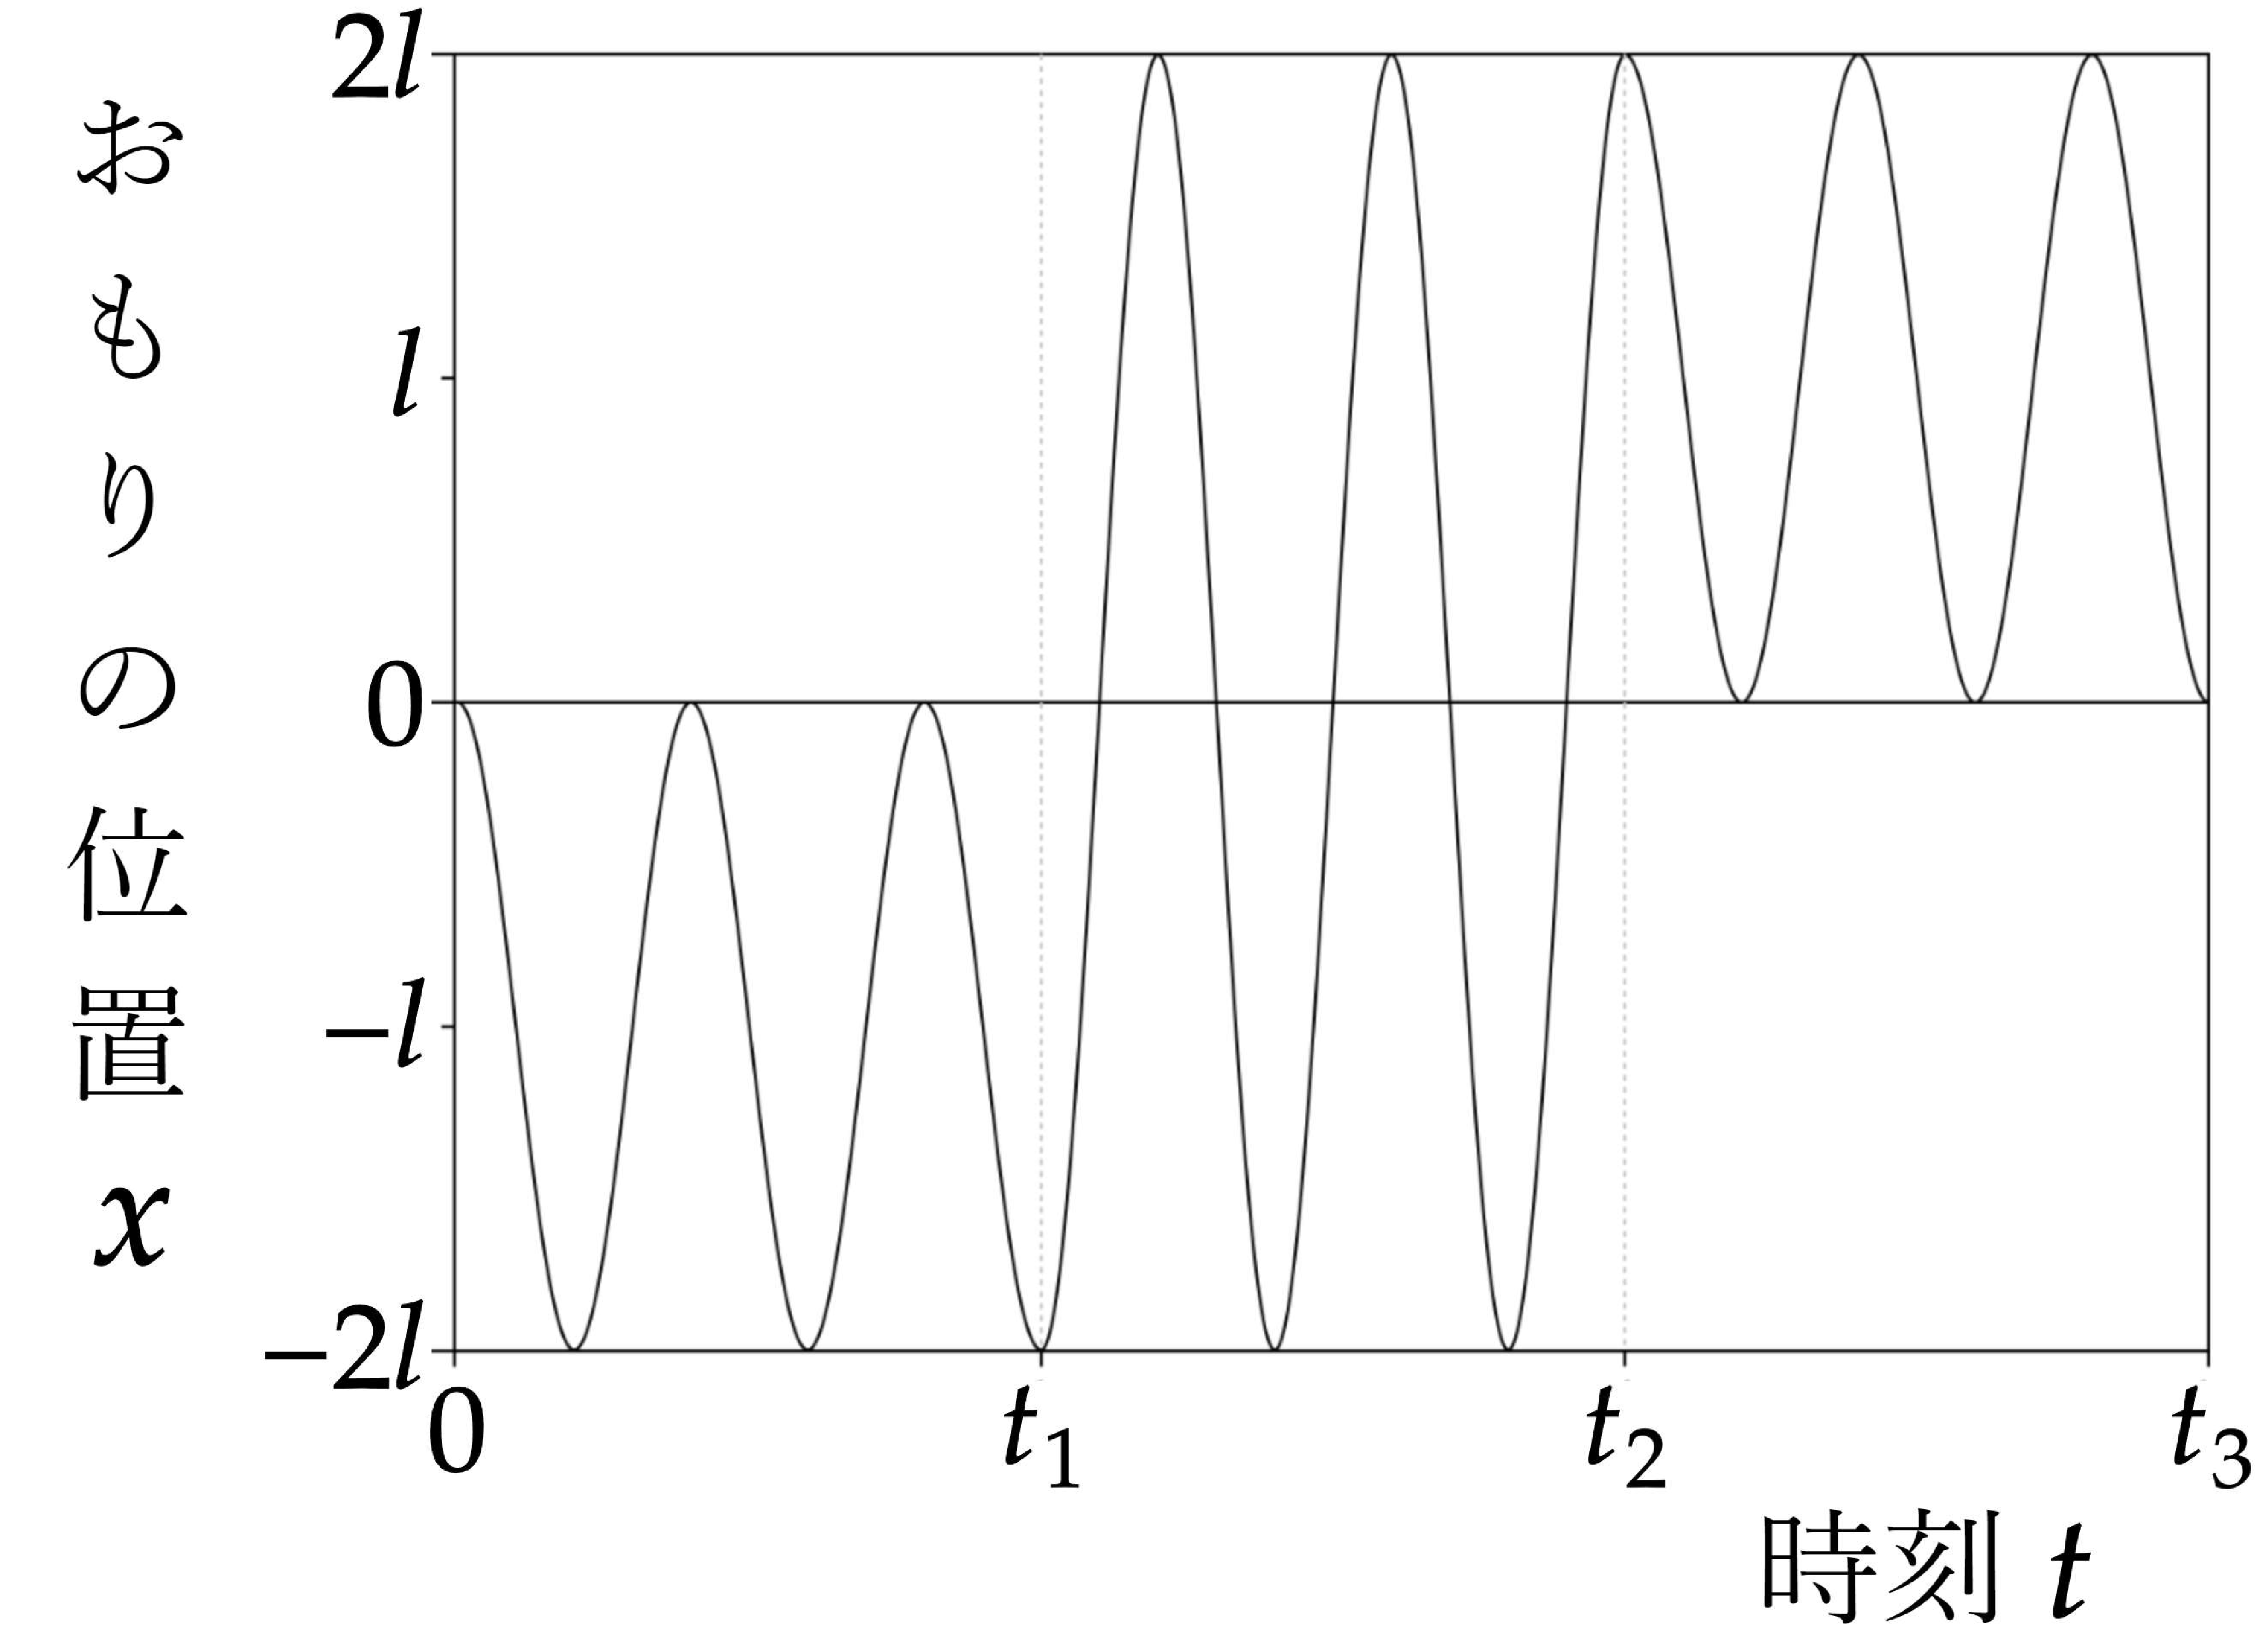
\includegraphics[width=6cm]{fig/fig_1_7_2.pdf}
      \caption{}
    \end{figure}
    \end{minipage}
    \vspace{1em}
    \item {\hzw}\textbf{問2}において,時刻$t = 0 \sim t_1$の間に電車が加速度計に対してした仕事を,$t_1$,$t_2$,$t_3$を用いずに表せ.
    \item {\hzw}\textbf{問2}において,時刻$t  = 0 \sim t_3$の間,加速度計を床に固定しなくても加速度計がすべり出さないための条件を求めよ.ただし,床と加速度計の間の静止摩擦係数$\mu$は,おもりの位置によらず一定であるとする.
  \end{enumerate}
  \item {\hzw}図3に示すように,電車が傾斜角$\theta$の斜面上で停止し,おもりがつり合いの位置で静止している状態から,時刻$t = 0$以降において,電車が一定の加速度$a$で斜面を登る場合を考える.
  \begin{figure}[H]
    \centering
    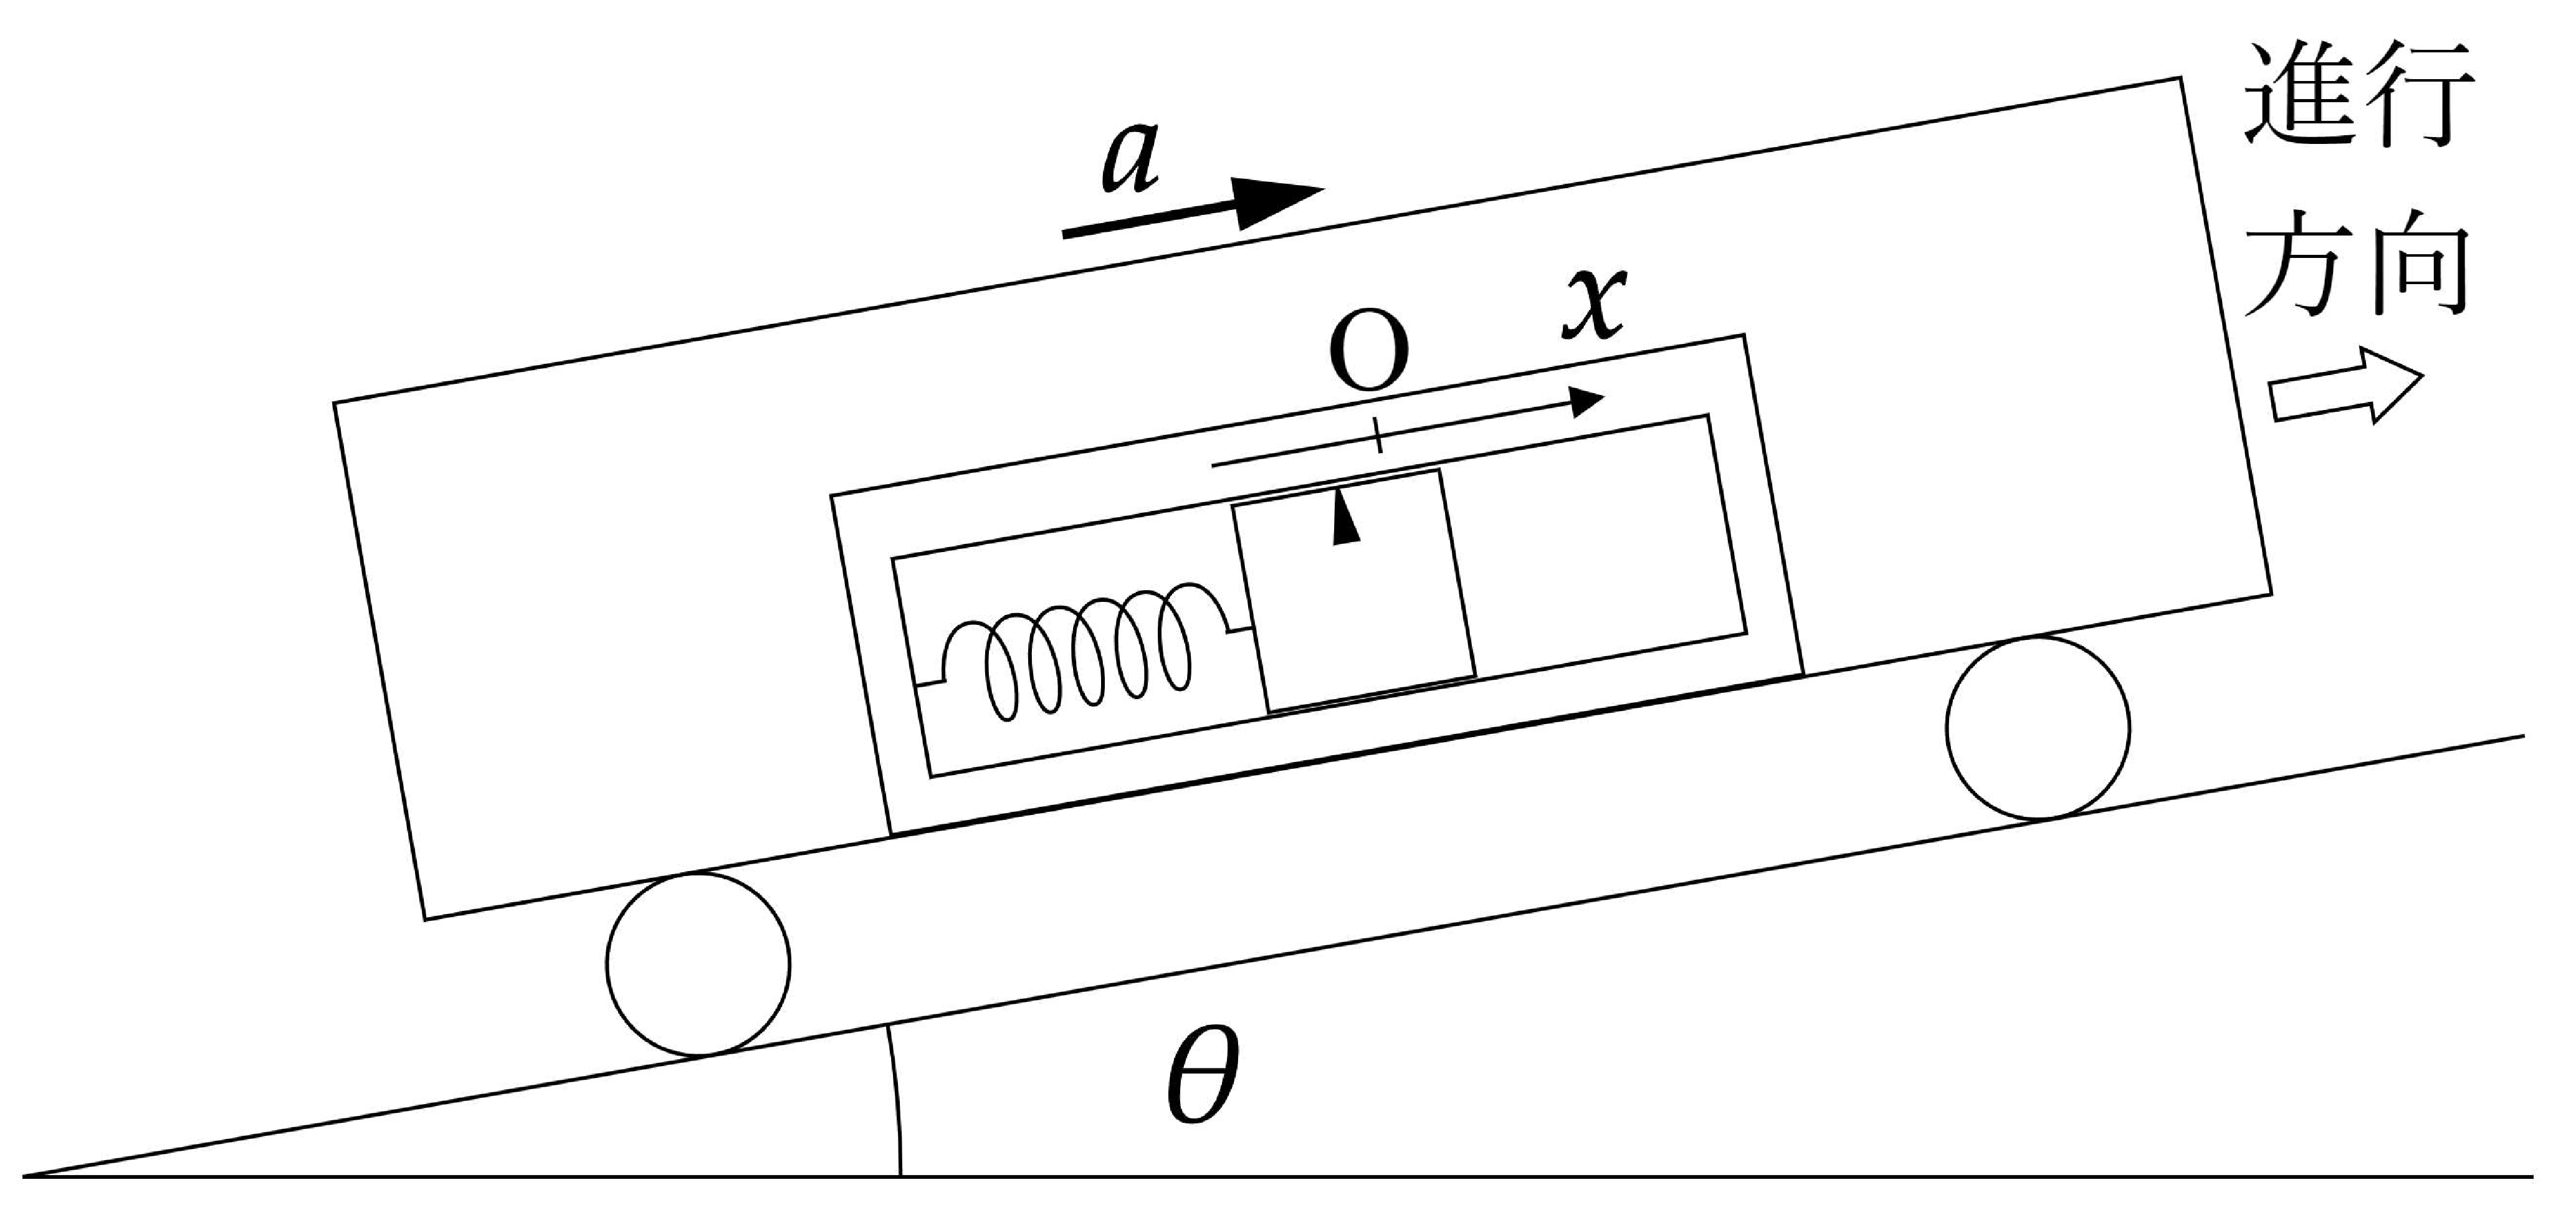
\includegraphics[width=7cm]{fig/fig_1_7_3.pdf}
    \caption{}
  \end{figure}
  \begin{enumerate}[resume, label=\textbf{問\arabic*}]
    \item {\hzw}時刻$t$とおもりの位置$x$の関係を,グラフおよび数式で表せ.
    \item {\hzw}時刻$t = t_4$で,電車の運動は等速直線運動に変わった.$t > t_4$において,おもりが枠に対して静止し続けるための$t_4$の条件を求めよ.
  \end{enumerate}
\end{enumerate}

\end{document}